\section{Empirical Evaluation}
\label{sec:evaluation}

Operating our causal measurement platform across all five browser configurations, our testbed completed crawls over all 150 curated publisher domains across both phases ($100.0\%$ completion yield). 
Table~\ref{tab:master_results} presents the empirical results structured across our three measurement silos: economic bid valuation, network identity diffusion, and client-side usability overheads.

\begin{table*}[t]
\centering
\small
\caption{Master Empirical Evaluation Matrix across 150 Commercial Publishers. 
Absolute bids reflect Pre/Post medians; $\Delta\cpm$ distributions show first quartile ($Q_1$), median, and third quartile ($Q_3$); Identity Diffusion decomposes into Cookie Syncs ($S_{\text{post}}$) and Smuggled UIDs ($U_{\text{post}}$); Usability Cost ($\ucost$) is normalized to the Chrome control group.}
\label{tab:master_results}
\resizebox{\textwidth}{!}{%
\setlength{\tabcolsep}{4pt}
\begin{tabular}{lcccccccccccc}
\toprule
\textbf{Configuration} & $|\mathcal{S}_{\text{active}}|$ & \textbf{Pre \$} & \textbf{Post \$} & $\rid$ & \textbf{Spread ($Q_1$ / Med / $Q_3$)} & \textbf{IQR} & $S_{\text{post}}$ & $U_{\text{post}}$ & $D_{\text{ID}}$ & $\ucost$ & \textbf{Wilcoxon $W$ ($p$)} & $\etr$ \\
\midrule
\texttt{chrome\_baseline}  & 33 & \$0.08 & \$0.05 & 0.606 & -75.00\% / \textbf{-1.12\%} / +123.11\% & 198.11\% & 3,206 & 18,359 & 21,565 & 0.00 & 226.5 ($p=0.4832$) & 0.105 \\
\texttt{firefox\_baseline} & 46 & \$0.09 & \$0.05 & 0.543 & -99.30\% / \textbf{-4.11\%} / +106.19\% & 205.49\% & 2,461 & 18,414 & 20,875 & 0.00 & 414.0 ($p=0.3445$) & 0.136 \\
\texttt{brave\_baseline}   & 41 & \$0.15 & \$0.08 & 0.537 & -100.0\% / \textbf{-21.39\%} / +46.95\% & 146.95\% & 3,302 & 18,515 & 21,817 & 0.31 & 345.0 ($p=0.5300$) & 0.131 \\
\texttt{firefox\_hardened} & 54 & \$0.09 & \textbf{\$0.02} & 0.574 & -99.86\% / \textbf{-26.86\%} / \textbf{+1.20\%} & 101.06\% & 6,006 & 22,970 & 28,976 & 0.00 & 472.0 ($p=\textbf{0.0734}$) $\dagger$ & 0.175 \\
\texttt{brave\_hardened}   & 46 & \$0.15 & \textbf{\$0.06} & \textbf{0.500} & -100.0\% / \textbf{-59.98\%} / \textbf{0.00\%} & \textbf{100.00\%} & 3,229 & 18,885 & 22,114 & \textbf{0.44} & 361.5 ($p=0.1192$) & \textbf{0.179} \\
\bottomrule
\end{tabular}%
}
\vspace{1pt}
\flushleft{\footnotesize $\dagger$ Statistically significant at the marginal $\alpha = 0.10$ level. Omnibus Kruskal-Wallis across all 5 configurations: $H = 7.570$, $p = 0.1087$.}
\end{table*}

\subsection{Dataset Integrity \& CMP Consent Yield}
\label{subsec:observability_yield}

Applying the Paired Observability Filter (Section~\ref{subsec:curation}) extracted between 33 and 54 actively observable publisher auctions per configuration ($22.0\%$ to $36.0\%$ Prebid transparency). 

As established in prior header bidding measurements~\cite{pachilakis2019no, cook2020inferring}, client-side wrappers capture the observable portion of programmatic inventory; unobserved domains either route auctions through opaque Server-to-Server (S2S) frameworks (e.g., Google Open Bidding, Amazon TAM) or experienced exchange timeouts exceeding our 15.0-second collection window. 

Crucially, the 3-Tier Consent Clicker successfully negotiated European privacy gates across the crawl:
\begin{itemize}
    \item \texttt{chrome\_baseline}: 107 domains resolved ($71.3\%$ auto-accepted; 61 regex, 43 CSS, 3 API);
    \item \texttt{firefox\_hardened}: 118 domains resolved ($78.7\%$ auto-accepted; 64 regex, 53 CSS, 1 API);
    \item \texttt{brave\_hardened}: 114 domains resolved ($76.0\%$ auto-accepted; 59 regex, 51 CSS, 4 API).
\end{itemize}
The unhandled minority ($21.3\%$--$32.0\%$) comprised non-EU sites lacking consent banners or publishers serving custom, non-standard modal overlays~\cite{papadogiannakis2021user}.

\subsection{Silo 1: Economic Valuation Analysis}
\label{subsec:silo_econ}

Figure~\ref{fig:iqr_spread} plots the full distributional spread of relative bid shifts across configurations, demonstrating how defensive hardening compresses market valuation.

\begin{figure}[t]
\centering
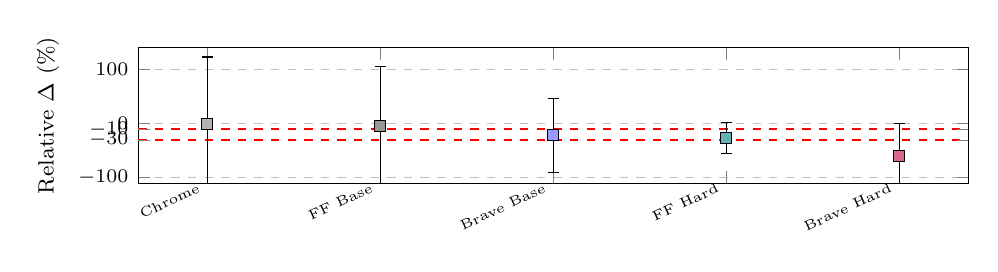
\begin{tikzpicture}
\begin{axis}[
    width=\columnwidth,
    height=3.3cm,
    ymin=-110, ymax=140,
    ylabel={Relative $\Delta\cpm$ (\%)},
    ylabel style={font=\footnotesize},
    ticklabel style={font=\scriptsize},
    symbolic x coords={Chrome, FF Base, Brave Base, FF Hard, Brave Hard},
    xtick={Chrome, FF Base, Brave Base, FF Hard, Brave Hard},
    x tick label style={rotate=25, anchor=east, font=\tiny},
    ymajorgrids=true,
    grid style=dashed,
    extra y ticks={-10, -30},
    extra y tick style={grid=major, grid style={red, dashed, line width=0.8pt}}
]
% Box plots via error bars: Q1 to Q3, with median marks
\addplot+[black, mark=square*, mark options={fill=gray!60}, error bars/.cd, y dir=both, y explicit] 
    coordinates {(Chrome, -1.12) +- (73.88, 124.23)};
\addplot+[black, mark=square*, mark options={fill=gray!80}, error bars/.cd, y dir=both, y explicit] 
    coordinates {(FF Base, -4.11) +- (95.19, 110.30)};
\addplot+[black, mark=square*, mark options={fill=blue!40}, error bars/.cd, y dir=both, y explicit] 
    coordinates {(Brave Base, -21.39) +- (78.61, 68.34)};
\addplot+[black, mark=square*, mark options={fill=teal!60}, error bars/.cd, y dir=both, y explicit] 
    coordinates {(FF Hard, -26.86) +- (73.00, 28.06)};
\addplot+[black, mark=square*, mark options={fill=purple!60}, error bars/.cd, y dir=both, y explicit] 
    coordinates {(Brave Hard, -59.98) +- (40.02, 59.98)};
\end{axis}
\end{tikzpicture}
\caption{Distributional spread of relative price shifts ($\Delta\cpm$) across configurations. Points indicate median values; error bars denote the Interquartile Range ($Q_1$ to $Q_3$). Red dashed lines indicate the $-10\%$ noise and $-30\%$ \htr boundaries.}
\label{fig:iqr_spread}
\end{figure}

\paragraph{Negative Control \& Default Defenses}
In unhardened Chrome, state purging produces a median bid shift of only $-1.12\%$ ($p = 0.4832$, fail to reject $H_0$), with $60.61\%$ of publishers re-identifying the client within market noise ($\rid = 0.606$). 
While isolated domains experience bid drops (e.g., \url{allrecipes.com}, $\$10.00 \to \$0.00$), others clear at elevated rates (e.g., \url{archdaily.com}, $\$26.00$), demonstrating empirically that commercial DSPs routinely bridge storage resets via stateless graphs~\cite{acar2014web, liu2025first}. 
Default browser protections offer negligible resistance: standard Firefox yields a median shift of $-4.11\%$ ($p = 0.3445$, $\rid = 0.543$), as static ETP blocklists fail to restrict active canvas or audio readbacks. 
While default Brave farbling induces valuation uncertainty ($\Delta\cpm = -21.39\%$, median $\$0.15 \to \$0.08$) through algorithmic bid shading~\cite{barysei2023investigating}, its wide dispersion ($Q_3 = +46.95\%$, $\rid = 0.537$) confirms that cross-session graph linkage remains largely intact.

\paragraph{Hardened Defenses: Normalization vs.\ Disruption}
Hardened configurations alter auction dynamics substantially, establishing two distinct operational profiles. Hardened Firefox achieves a $-26.86\%$ median bid collapse ($p = 0.0734$, $W = 472.0$), driving the median clearing bid from $\$0.09$ down to $\$0.02$ ($77.8\%$ decline) with the upper quartile compressed to $Q_3 = +1.20\%$. 
Crucially, Tor-derived RFP normalization achieves this disruption with zero client-side script breakage ($\ucost = 0.00$). In contrast, Hardened Brave enforces the most aggressive economic intervention: median bids collapse by $-59.98\%$ ($\$0.15 \to \$0.06$, $\rid = 0.500$). 
Its lower quartile drops to complete bid suppression ($Q_1 = -100.0\%$, with domains like \url{dailymail.co.uk} and \url{cricbuzz.com} falling to $\$0.00$), while the upper quartile is capped at $Q_3 = 0.00\%$, indicating non-positive bid shifts across $75\%$ of active inventory. 
However, this tracking severance comes at the expense of severe script dependency breakage ($\ucost = 0.44$).

\subsection{Ad-Tech Pricing \& Non-Parametric Rank Dilution}
\label{subsec:rank_dilution}

Despite Brave Hardened's $-59.98\%$ median collapse and $Q_3 \le 0.00\%$ compression, its paired Wilcoxon test yielded $W = 361.5$ ($p = 0.1192$). 
This statistical artifact stems from two structural properties of programmatic ad markets~\cite{barysei2023investigating}: 
(1)~\textit{Left-censored reserve floors} ($\$0.01$--$\$0.05$) truncate negative differences ($|D_i| \le \$0.15$); and 
(2)~\textit{heteroskedastic video outliers} heavily penalize signed-rank sums. 
Because the Wilcoxon test ranks observations by absolute dollar difference ($|D_i|$), isolated outstream video ad spikes (e.g., $\$0.04 \to \$16.00$ on \url{standard.co.uk}, and $\$0.10 \to \$22.00$ on \url{verywellhealth.com}) receive maximum ranks ($R_i = N$), counterbalancing dozens of consistent display ad collapses ($-\$0.50$). 
Per ASA inference guidelines~\cite{wasserstein2016asa}, real-world economic significance in high-variance financial auctions must be evaluated via effect size and quartile compression ($Q_3 \le 0.00\%$) rather than rank-sum symmetry alone.

\subsection{Silo 2: Identity Diffusion \& The Retry Storm}
\label{subsec:silo_network}

While clearing prices reveal identity certainty from the buyer's perspective, inspecting underlying network flows demonstrates how browser defenses alter tracker coordination in the background.
Decomposing Identity Diffusion ($D_{\text{ID}}$) into Cookie Synchronizations ($S_{\text{post}}$)~\cite{papadopoulos2019cookie} and Smuggled Navigational Identifiers ($U_{\text{post}}$)~\cite{randall2022measuring} reveals an unexpected operational divergence across configurations:
Across \texttt{chrome\_baseline}, \texttt{firefox\_baseline}, and both Brave configurations, syncs and smuggled UIDs remained remarkably stable: $S_{\text{post}} \in [2,461, 3,302]$ and $U_{\text{post}} \in [18,359, 18,885]$.
In stark contrast, \texttt{firefox\_hardened} exhibited a pronounced surge: \textbf{Cookie Synchronizations more than doubled to $S_{\text{post}} = 6,006$}, and \textbf{Smuggled UIDs surged to $U_{\text{post}} = 22,970$}, driving total diffusion events to $D_{\text{ID}} = 28,976$. 
Inspection of proxy logs reveals this was driven by a \textbf{stateless blocking retry storm}: when Firefox's multi-layered defenses (Total Cookie Protection, RFP canvas blanking, and query parameter stripping) blocked tracker endpoints and sanitized link decorations, client-side tracking scripts threw exceptions and repeatedly re-triggered synchronization requests within recursive event loops~\cite{iqbal2020adgraph}. 
Crucially, deduplicating target endpoints revealed that Hardened Firefox communicated with the fewest distinct tracking hosts (\textbf{810 hosts}, vs. 872 in Chrome and 888 in Brave Hardened). Thus, while request \textbf{frequency} spiked due to client-side retries, Firefox successfully restricted the \textbf{diffusion} of identifiers across unique commercial entities.

\subsection{Silo 3: Usability Cost \& Runtime Breakage}
\label{subsec:silo_usability}

While normalized defenses contained entity diffusion without modifying DOM layouts, blocking network requests introduced measurable client-side breakage.

Client-side error logging captured 45,000+ unhandled runtime JavaScript exceptions across our crawls. Cross-engine normalization reveals key differences between defense approaches:
\begin{itemize}
    \item \textbf{Gecko Engine Performance:} Standard Firefox recorded 1,590 exceptions, while Hardened Firefox recorded 2,400 exceptions ($+50.9\%$). 
However, because RFP's timer quantization and canvas blanking return syntactically valid mock objects, these errors did not alter DOM layout trees or break page scripts, preserving a usability penalty of $\ucost = 0.00$.
    \item \textbf{Chromium Engine Performance:} Chrome Baseline recorded 12,816 exceptions. Brave Baseline logged 13,309 exceptions ($\ucost = 0.31$), and Brave Hardened logged 14,882 exceptions ($\ucost = 0.44$).
\end{itemize}

Brave's aggressive network-layer request blocking severs script dependency chains, causing downstream publisher scripts to throw unhandled \texttt{TypeError} and null-pointer exceptions that degrade site features~\cite{iqbal2020adgraph}. 
These empirical results reveal an operational paradox: defensive blocking triggers network retry storms that artificially inflate raw request counts, while aggressive filtering incurs substantial usability breakage. In Section~\ref{sec:discussion}, we deconstruct how naive composite metrics fail to capture these trade-offs, motivating the formulation of $\etr$.